\documentclass{article}

\usepackage[utf8]{inputenc}
\usepackage[margin=3cm]{geometry}
\usepackage{graphicx}
\usepackage{minted}
\usepackage{xcolor}
\usepackage{hyperref}
\usepackage{caption}
\usepackage{amsmath}
\usepackage[backend=bibtex, style=authoryear]{biblatex}

\hypersetup{colorlinks,linkcolor=,urlcolor=,citecolor=blue}
\usemintedstyle{friendly}
\definecolor{bg}{rgb}{0.95,0.95,0.95}
\addbibresource{references.bib}

\title{Lab 06: A ``gentle'' Introduction to Support Vector Machines in R}
\author{Andrés Oswaldo Calderón Romero, PhD.}
\date{\today}

\begin{document}

\maketitle

\section{Introduction}
Support Vector Machines (SVMs) offer a powerful approach to binary classification by attempting to find a \textbf{hyperplane} in a feature space that ``best'' separates two classes. While perfect linear separation is often impossible in the original feature space, SVMs extend this concept by softening the separation requirements and using the \textbf{kernel trick} to enlarge the feature space, making separation more likely.

\section{The Kernel Trick}
When classes are not linearly separable, SVMs use \textbf{kernel functions} to project data into a higher-dimensional space where a linear hyperplane can separate them. Common kernels include:

\begin{itemize}
    \item \textbf{Polynomial}: $K(x, x') = (1 + \langle x, x' \rangle)^d$

    \item \textbf{Radial Basis Function (RBF)}: $K(x, x') = \exp(-\gamma ||x - x'||^2)$

    \item \textbf{Hyperbolic Tangent}: $K(x, x') = \tanh(\kappa_1 ||x - x'|| + \kappa_2)$
\end{itemize}

\section{Implementation in R}
Although there are a number of great packages that implement SVMs (e.g., e1071 \parencite{meyer2019e1071} and svmpath \parencite{hastie2016svmpath}), we’ll focus on the most flexible implementation of SVMs in R: kernlab \parencite{karatzoglou2004kernlab}. We’ll also use caret for tuning SVMs and pre-processing. In this chapter, we’ll explicitly load the following packages:

\begin{listing}[H]
    \begin{minted}[
    frame=lines,
    framesep=2mm,
    baselinestretch=1.2,
    bgcolor=bg,
    fontsize=\footnotesize
    ]{r}
# Helper packages
library(dplyr)    # for data wrangling
library(ggplot2)  # for awesome graphics
library(modeldata)  # for data access and splitting

# Modeling packages
library(caret)    # for classification and regression training
library(kernlab)  # for fitting SVMs

# Model interpretability packages
library(pdp)      # for partial dependence plots, etc.
library(vip)      # for variable importance plots
    \end{minted}
    \caption{Package Initialization: Loading essential libraries for data wrangling, visualization, and SVM modelling.}
\end{listing}

To illustrate the basic concepts of fitting SVMs we’ll use a mix of simulated data sets as well as the employee attrition data. The code for generating the simulated data sets and figures in this chapter are available on the book website. In the employee attrition example our intent is to predict on Attrition (coded as ``Yes''/``No''). As in previous labs, we’ll set aside 30\% of the data for assessing generalizability.

\begin{listing}[H]
    \begin{minted}[
    frame=lines,
    framesep=2mm,
    baselinestretch=1.2,
    bgcolor=bg,
    fontsize=\footnotesize
    ]{r}
# Load attrition data
df <- attrition %>%
  mutate_if(is.ordered, factor, ordered = FALSE)

# Create training (70%) and test (30%) sets
set.seed(42)  # for reproducibility
churn_split <- initial_split(df, prop = 0.7, strata = "Attrition")
churn_train <- training(churn_split)
churn_test  <- testing(churn_split)
    \end{minted}
    \caption{Data Preparation: Formatting the ``attrition'' dataset and partitioning it into 70\% training and 30\% testing sets.}
\end{listing}

Notice how each of these kernel functions include hyperparameters that need to be tuned. For example, the polynomial kernel includes a degree term $d$ and a scale parameter  $\gamma$. Similarly, the radial basis kernel includes a $\gamma$ parameter related to the inverse of the $\sigma$ parameter of a normal distribution. In R, you can use caret’s \texttt{getModelInfo()} to extract the hyperparameters from various SVM implementations with different kernel functions, for example:

\begin{listing}[H]
    \begin{minted}[
    frame=lines,
    framesep=2mm,
    baselinestretch=1.2,
    bgcolor=bg,
    fontsize=\footnotesize
    ]{r}
# Linear (i.e., soft margin classifier)
caret::getModelInfo("svmLinear")$svmLinear$parameters
##   parameter   class label
## 1         C numeric  Cost

# Polynomial kernel
caret::getModelInfo("svmPoly")$svmPoly$parameters
##   parameter   class             label
## 1    degree numeric Polynomial Degree
## 2     scale numeric             Scale
## 3         C numeric              Cost

# Radial basis kernel
caret::getModelInfo("svmRadial")$svmRadial$parameters
##   parameter   class label
## 1     sigma numeric Sigma
## 2         C numeric  Cost
    \end{minted}
    \caption{Hyperparameter Discovery: Identifying tunable parameters (e.g., $C$, $degree$, and $\sigma$) for Linear, Polynomial, and RBF kernels.}
\end{listing}

We utilize the \texttt{kernlab} package for fitting SVMs and \texttt{caret} for hyperparameter tuning.  The plotting results can be seen in Figure~\ref{fig:attrition_svm}.

\begin{listing}[H]
    \begin{minted}[
    frame=lines,
    framesep=2mm,
    baselinestretch=1.2,
    bgcolor=bg,
    fontsize=\footnotesize
    ]{r}
# Example: Training an SVM with a Radial Basis Kernel
# 'attrition' dataset assumed to be pre-loaded

# Tune an SVM with radial basis kernel

set.seed(42)
churn_svm <- train(
    Attrition ~ .,
    data = churn_train,
    method = "svmRadial",
    preProcess = c("center", "scale"),
    trControl = trainControl(method = "cv", number = 10),
    tuneLength = 10
)

# View tuning results
print(churn_svm$results)

#          sigma      C  Accuracy     Kappa  AccuracySD   KappaSD
# 1  0.009788409   0.25 0.8395141 0.0000000 0.004205199 0.0000000
# 2  0.009788409   0.50 0.8395141 0.0000000 0.004205199 0.0000000
# 3  0.009788409   1.00 0.8590082 0.1906199 0.015478150 0.1114105
# 4  0.009788409   2.00 0.8833002 0.4301047 0.027982904 0.1551574
# 5  0.009788409   4.00 0.8842998 0.4693976 0.029904716 0.1644876
# 6  0.009788409   8.00 0.8794357 0.4750025 0.030505379 0.1589090
# 7  0.009788409  16.00 0.8706501 0.4515783 0.031627149 0.1538052
# 8  0.009788409  32.00 0.8696886 0.4537813 0.027796066 0.1413571
# 9  0.009788409  64.00 0.8687177 0.4518817 0.029981421 0.1452463
# 10 0.009788409 128.00 0.8687177 0.4518817 0.029981421 0.1452463

# Plot results
g <- ggplot(churn_svm) + theme_light()
plot(g)
    \end{minted}
    \caption{SVM Implementation: Training a Radial Basis Function (RBF) model with 10-fold cross-validation and hyperparameter optimization.}\end{listing}

\begin{figure}
 \centering
 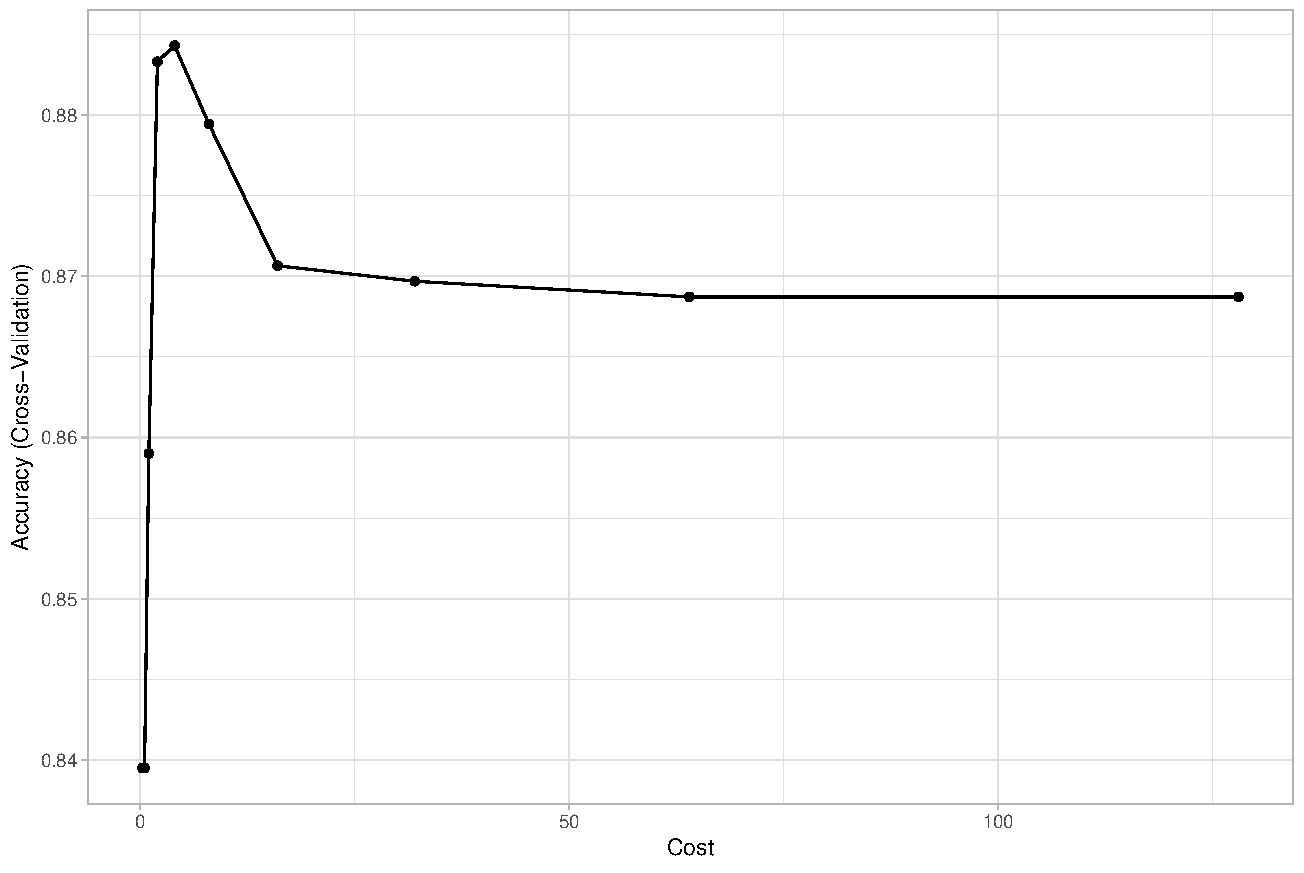
\includegraphics[width=0.75\textwidth]{figures/attrition_svm.pdf}
 % attrition_svm.pdf: 626x419 px, 72dpi, 22.08x14.78 cm, bb=0 0 626 419
 \caption{Plotting the results, we see that smaller values of the cost parameter ($C\approx2–8$) provide better cross-validated accuracy scores for these training data.}
 \label{fig:attrition_svm}
\end{figure}

\section{Autonomous Work}
Reproduce the Support Vector Machine (SVM) implementation using the ``Advertisement'' dataset as detailed in Section 3 of Lab 05. Specifically, you are required to:

\begin{enumerate}
    \item \textbf{Data Partitioning:} Load the dataset and perform a 75/25 training/testing split.
    \item \textbf{Feature Scaling:} Standardize the ``Age'' and ``EstimatedSalary'' variables.
    \item \textbf{Model Fitting:} Train an SVM classifier using the \texttt{ksvm} function from the \texttt{kernlab} package or the \texttt{train} function from \texttt{caret}.
    \item \textbf{Kernel Evaluation:} Evaluate model performance across various kernels (Linear, Polynomial, and RBF) and report the resulting accuracy for each.
    \item \textbf{Performance Analysis:} Generate a confusion matrix and calculate validation metrics. Compare these results with the performance of the Decision Tree model developed in the previous lab.
\end{enumerate}

\printbibliography[title={References}]

\end{document}
